%%%%%%%%%%%%%%%%%%%%%%%%%%%%%%%%%%%%%%%%%
% Friggeri Resume/CV
% XeLaTeX Template
% Version 1.2 (3/5/15)
%
% This template has been downloaded from:
% http://www.LaTeXTemplates.com
%
% Original author:
% Adrien Friggeri (adrien@friggeri.net)
% https://github.com/afriggeri/CV
%
% License:
% CC BY-NC-SA 3.0 (http://creativecommons.org/licenses/by-nc-sa/3.0/)
%
% Important notes:
% This template needs to be compiled with XeLaTeX and the bibliography, if used,
% needs to be compiled with biber rather than bibtex.
%
%%%%%%%%%%%%%%%%%%%%%%%%%%%%%%%%%%%%%%%%%

\documentclass[]{friggeri-cv} % Add 'print' as an option into the square bracket to remove colors from this template for printing
\usepackage{graphicx}
\graphicspath{ {images/} }

\begin{document}

\header{Stefano}{Munarini}{Computer Science graduate student} % Your name and current job title/field

%----------------------------------------------------------------------------------------
%	SIDEBAR SECTION
%----------------------------------------------------------------------------------------

\begin{aside} % In the aside, each new line forces a line break
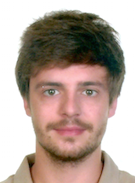
\includegraphics[scale=0.5]{fototessera}
\section{contact}
Via Bregonze, 17
Thiene, 36016
Italy
+39 340 691 7486
\href{mailto:stefano.munarini@me.com}{stefano.munarini@me.com}
Skype: stestisa
\href{https://github.com/stestisa}{GitHub: stestisa}
\href{https://it.linkedin.com/in/munarinistefano}{LinkedIn: munarinistefano}
\href{http://stackexchange.com/users/2741833/stefano-munarini}{StackOverflow: 2741833}
\section{languages}
Italian mother tongue
English proficient
\section{programming}
\textbf{Academic:} Java, C++,
SQL, HTML
\textbf{Personal:} Python, Swift,
Javascript, LaTeX
%--Java, Swift, Python,
%C++, Javascript,
%SQL, LaTeX, HTML
\end{aside}

%----------------------------------------------------------------------------------------
%	ABOUT ME SECTION
%----------------------------------------------------------------------------------------


\section{about me}
{I am an Italian graduate student with a bachelor degree in Computer Science achieved in 2015 at the University of Trento. I live in Vicenza with my family but I’m traveling around Europe for studying and working purposes.
\\
I consider myself as a young digital entrepreneur constantly looking for innovation in the field of information technology (IT). I am very ambitious and that is why I always succeed in what I do.
\\
I am cut out to be a team-leader, to share my visions and to develop them with others.
I never force anyone into a different direction without having discussed it before. That is the reason why I care a lot about others’ opinion: I reckon that sharing and then modeling a thought with someone drives to a better solution. 
\\
I am a really open minded person who approaches the views and knowledge of others to improve personal and professional skills.
}

%----------------------------------------------------------------------------------------
%	WORK EXPERIENCE SECTION
%----------------------------------------------------------------------------------------

\section{experience}

\subsection{Internship}

{Feb 2014 -- Jun 2014} \\
{\textbf{Java Developer}} \\
{\href{http://www.dedagroup.it}{Dedagroup ICT Network}} -- {Trento, Italy} \\
{During the internship I had the chance to improve my skills as a software engineer (see \textit{HEMME} in project section). In particular, I improved my Java skills and became able to develop a backend using the Spring Framework. In addition, I enhanced my team-working and communication skills, thanks to the involvement in an international team. Furthermore, I became more competent as an Android developer, gaining professional knowledge in particular with geo-localization and background services.
\\
Detailed achievements:
\begin{itemize}
\item I was able to solve complex problems the team had, avoiding therefore to waste time.
\item I improved team productivity by sharing my knowledges, in particular with Android design and development.
\item I leaded the team to the completion of the project, setting daily briefs where we used to discuss how to split the work between team members and how to proceed with the tasks development.
\end{itemize}}

%----------------------------------------------------------------------------------------

%\subsection{Part Time}

%{May 2013 -- Nov 2013} \\
%{\textbf{Software Tester}} \\
%{\href{http://www.inria.fr}{Inria}} -- {Trento Area, Italy} \\
%{During this period I have tested and reported bugs to developers about the Web and the mobile application \emph{AllYours}.} \\

%----------------------------------------------------------------------------------------
%	PROJECT SECTION
%----------------------------------------------------------------------------------------

\section{projects}

{Jul 2013 -- Now} \\
{\href{https://play.google.com/store/apps/details?id=com.povodev.libretto}{\textbf{Libretto Universitario}}} \\
{This is an Android application with over 80K downloads which aims at simplifying the management and the organization of students' academic career. As a matter of fact this application allows not only to compute the arithmetic mean and the degree grade, but also to see detailed statistics (such as charts, year-by-year marks trend), to plan future exams, to organize a timetable and to have a record of all payed taxes. \\
This application has been developed with easy-of-use in mind, thus respecting Usability's Nielsen principle, with a graphic carefully and properly designed.} \\
{Technologies used: Java, SQL, Android, Parse} \\

%------------------------------------------------

{Feb 2014 -- Jun 2014} \\
{\textbf{HEMME}} \\
{Internship project - Dedagroup ICT Network} \\
{The goal of this project was to develop and to implement a mobile application, supported by a backend, that can help people affected by Alzheimer's Disease, their tutors and their doctors.} \\
{Technologies used: Java2EE, SQL, Spring framework, Android} \\

%------------------------------------------------

{Oct 2013 -- Dec 2013} \\
{\href{https://github.com/stestisa/StudentsChat}{\textbf{Student's Chat}}} \\
{University project (\textit{Introduction to Web Programming} course, mark: 28/30)} \\
{The goal of this project was to implement a web application where students can exchange ideas and educational materials (homeworks, notes, exam solutions and even more) in a simple and convenient way.} \\
{Technologies used: JSP, Java Servlet, Java Filter, JSTL, HTML, SQL} \\

%------------------------------------------------

{Feb 2012 -- May 2012} \\
{\textbf{aMuse}} \\
{University project (\textit{Software Engineering} course, mark: 30/30)} \\
{The goal of this project was to implement an application in order to make a visit at the museum an unforgettable experience. This experience could even be enjoyed once the visit is over thanks to the creation of a book where all the favourite works of art are stored; in addition it can also be shared with family and friends.} \\
{This project is made up of a web application and an Android application.} \\
{Technologies used: Java Servlet, JSP, Android, SQL}

%----------------------------------------------------------------------------------------
%	AWARDS SECTION
%----------------------------------------------------------------------------------------

\section{awards}

{Dec 2013} \\
{\textbf{\href{http://www.upperapp.it}{UpperApp Festival} - 1\textsuperscript{st} Prize: Best Mobile Application developed by a student} \\
{Agorà Telematica} \\
\emph{Libretto Universitario} has been awarded as \textit{Best Mobile Application} at the UpperApp Festival 1\textsuperscript{st} Edition, a mobile applications contest for Italian students.}

%----------------------------------------------------------------------------------------
%	EDUCATION SECTION
%----------------------------------------------------------------------------------------

\section{education}

%\begin{entrylist}

%\entry
{2011 -- 2015} \\
\textbf{{Bachelor {\normalfont of Computer Science}}} \\
{University of Trento, Italy}


%----------------------------------------------------------------------------------------
%	CERTIFICATE SECTION
%----------------------------------------------------------------------------------------

\section{certifications}

{Apr 2015} \\
{\href{https://certs.duolingo.com/ud85gf8c}{\textbf{Duolingo Proficiency Exam} in English: Proficient}}

{2010} \\
{\textbf{ECDL}: European Computer Driving Licence}

%{2008} \\
%{\textbf{Trinity GESE}: B2 of the CEFR}

%----------------------------------------------------------------------------------------
%	INTERESTS SECTION
%----------------------------------------------------------------------------------------

\section{interests}

\textbf{professional:} software design, web and mobile application design and development
\textbf{personal:} travelling, photograpy, vinyls, cooking, running, hiking

\end{document}